\documentclass[12pt]{article}

% --- MLA-style page: Times 12pt, double-spaced, 1in margins, "LastName N" header
\usepackage[letterpaper,margin=1in]{geometry}
\usepackage[T1]{fontenc}
\usepackage{textcomp}
\usepackage{amsmath}
\IfFileExists{newtxtext.sty}{\usepackage{newtxtext}\usepackage[varbb]{newtxmath}}{\usepackage{mathptmx}}
\usepackage{setspace}
\doublespacing
\usepackage{graphicx}
\usepackage{booktabs}
\usepackage{caption}
\captionsetup{font=small,labelfont=bf,skip=4pt}
\usepackage{array}
\usepackage{enumitem}
\setlist[itemize]{leftmargin=1.5em,itemsep=0pt,topsep=2pt,parsep=0pt}
\usepackage{fancyhdr}
\pagestyle{fancy}
\fancyhf{}
\fancyhead[R]{Ginzburg \thepage}
\renewcommand{\headrulewidth}{0pt}
\setlength{\headheight}{15pt}
\setlength{\parindent}{0.5in}
\usepackage[hidelinks]{hyperref}
\usepackage{titlesec}
\titleformat{\section}{\normalfont\bfseries}{\thesection.}{0.5em}{}
\titleformat{\subsection}{\normalfont\bfseries}{}{0em}{}
\titlespacing{\section}{0pt}{10pt}{2pt}
\titlespacing{\subsection}{0pt}{8pt}{2pt}
\renewcommand{\thesection}{\arabic{section}}

\newcommand{\ga}{\ensuremath{\mathit{ga}}}
\newcommand{\gap}{\ensuremath{\mathit{gap}}}

\begin{document}

\begin{center}
{\bfseries Synthetic Fair-Value Strategy}\\[2pt]
Matthew Ginzburg
\end{center}

\vspace{4pt}

\section{Introduction}

A prediction-market contract is a binary claim that pays \$1.00 if an outcome
occurs and \$0.00 if it does not; before settlement it trades between those
bounds at whatever price buyers and sellers agree reflects the outcome's
probability. Polymarket US launched regulated, real-money contracts of this kind
in January 2026, and its coverage of the 2026 FIFA World Cup listed, for each
tracked player in each match, three separate contracts on a central limit order
book: at least one goal, at least one assist, and at least one goal-or-assist.
Each has its own order book and its own update cadence.

These three contracts are not independent instruments. Scoring a goal is one of
the ways to record a goal-or-assist, so the compound contract can never be worth
less than either single-stat leg:
\[
P(\text{goal} \cup \text{assist}) \;\geq\; \max\!\big(P(\text{goal}),\,P(\text{assist})\big).
\]
When the compound contract is quoted less actively than the legs that decompose
it, its price drifts below that floor. This is a pricing error the market makes
against itself, and it can be measured without taking a position. Across
157{,}595 simultaneously captured three-leg quotes, the compound bid falls below
the goals bid in 28.81\% of pre-kickoff observations, and the compound contract
carries a 3.81$\times$ wider spread and rests 5.6$\times$ less size than the
goals leg it can be priced against.

Whether that staleness reverts is a separate question, and it is tested rather
than assumed. Conditioning on positions entered while the compound contract was
cheap relative to its formula fair value, the mispricing narrows toward fair
value 63.0\% of the time, against 15.1\% under a volatility-matched random walk
($z = 6.94$, $p < 0.000001$). A second strategy trades confirmed public
events directly: when a goal, a substitution, or a final whistle makes one side
of a contract near-certain, a resting order on the other side has not yet
requoted, and whoever acts before the book adjusts is trading a latency gap.

This paper measures the inefficiency, tests whether it holds up as a
statistically significant effect, and asks whether either strategy actually
beats the market's own pricing or only moves faster than it. Only the patience
strategy does. The speed strategy is profitable, but it buys contracts already
priced near certainty, so its win rate is the arithmetic of those prices rather
than a measurable edge. Section 5 works through that distinction.

\section{Data Pipeline and Screening Architecture}

The analysis runs on an automated pipeline that finds pre-kickoff prop markets,
checks them, and tracks them, while keeping out repricing driven by news rather
than staleness. The goal is a clean sample of simultaneously observed three-leg
quotes and a measurement of how prices behave in the window where the compound
contract de-stales.

The pipeline runs unattended on Windows Task Scheduler and pulls from three data
sources. First, market and event data comes from Polymarket US's public gateway
API, which carries a live score and match clock on each event object. Second, the
account's own fills, balances, and settlements come from the authenticated
portfolio API, signed with an Ed25519 key over the message
\texttt{\{timestamp\}\{method\}\{path\}}. Third, the event timestamps used for
latency measurement come from neutral match reports (FIFA, ESPN, Al Jazeera),
never from Polymarket's own price data, which keeps the latency figures from
being circular.

Polling is tiered by time to kickoff: every twenty minutes beyond six hours out,
tightening to every sixty seconds inside the final thirty minutes. Markets are
discovered structurally rather than from a hand-maintained list. The set of
soccer leagues is pulled live from the platform's own sports endpoint, which
returned seventy leagues besides the World Cup as of 2026-08-08; each league's
games are then enumerated against the API.

A clean three-leg observation is recorded only when the goals, assists, and
goals-or-assists contracts for the same player can all be read from the same
market state in a single pass. Pairing the three legs at identical capture
timestamps yields 157{,}595 simultaneous observations, of which 124{,}571 fall in
the forty-eight hours before kickoff. This is the sample used throughout the
paper.

Every fill is reconciled at ingestion: each trade row's quantity is checked
against its cost divided by its price, and the local trade log is matched
one-to-one by trade identifier against a fully paginated pull of the account's
complete live history (392 trades). The trading client used for these reads
exposes only balance, position, and activity lookups, and cannot place orders.

\section{Signal Identification}

For a given player in a given match, let $g$, $a$, and \ga\ be the traded prices
of the ``1+ goals,'' ``1+ assists,'' and ``1+ goals-or-assists'' contracts. Under
a statistical-independence approximation, inclusion--exclusion gives a fair value
for the compound contract:
\[
P(\text{goal} \cup \text{assist}) = P(\text{goal}) + P(\text{assist}) - P(\text{goal} \cap \text{assist})
\;\approx\; g + a - g\,a .
\]
The signal is the difference between that fair value and the contract's actual
price:
\[
\gap \;=\; (g + a - g\,a) \;-\; \ga .
\]
A positive \gap\ means the compound contract is trading cheap relative to its own
legs, which is a buy signal. Across 208 clean pre-kickoff samples, \gap\ averaged
$+0.0106$ and exceeded $0.05$ in absolute value in 31 of 208 cases. On an
instrument priced between \$0.00 and \$1.00, that is a meaningful mispricing.

The reference constraint is the logical floor from Section 1: because a goal is
one route to a goal-or-assist, a correctly priced compound contract can never
trade below either single-stat leg. A violation of that inequality is a pricing
error that needs no model to identify, only three simultaneous quotes.

This is not a riskless arbitrage. The independence approximation carries model
risk in both directions: a goal is negatively correlated with the same player's
own assist, which pushes true $P(\text{goal} \cap \text{assist})$ below $g\,a$,
while a player heavily involved in attack has elevated odds of both outcomes for
reasons outside the formula. The strategy is statistical relative value with
adverse-selection exposure: a resting bid improved toward fair value can still be
filled by a counterparty who is better informed than the formula.

\section{Data Analysis}

Every snapshot of quotes and book depth is bucketed by time to kickoff. The four
figures below test the mechanisms the two strategies rely on.

\subsection{Spread and Resting Depth by Market Leg}

The plot below breaks out the mean bid--ask spread and the mean resting size for
each of the three legs, over the forty-eight hours before kickoff, for the
fourteen highest-coverage players.

\begin{center}
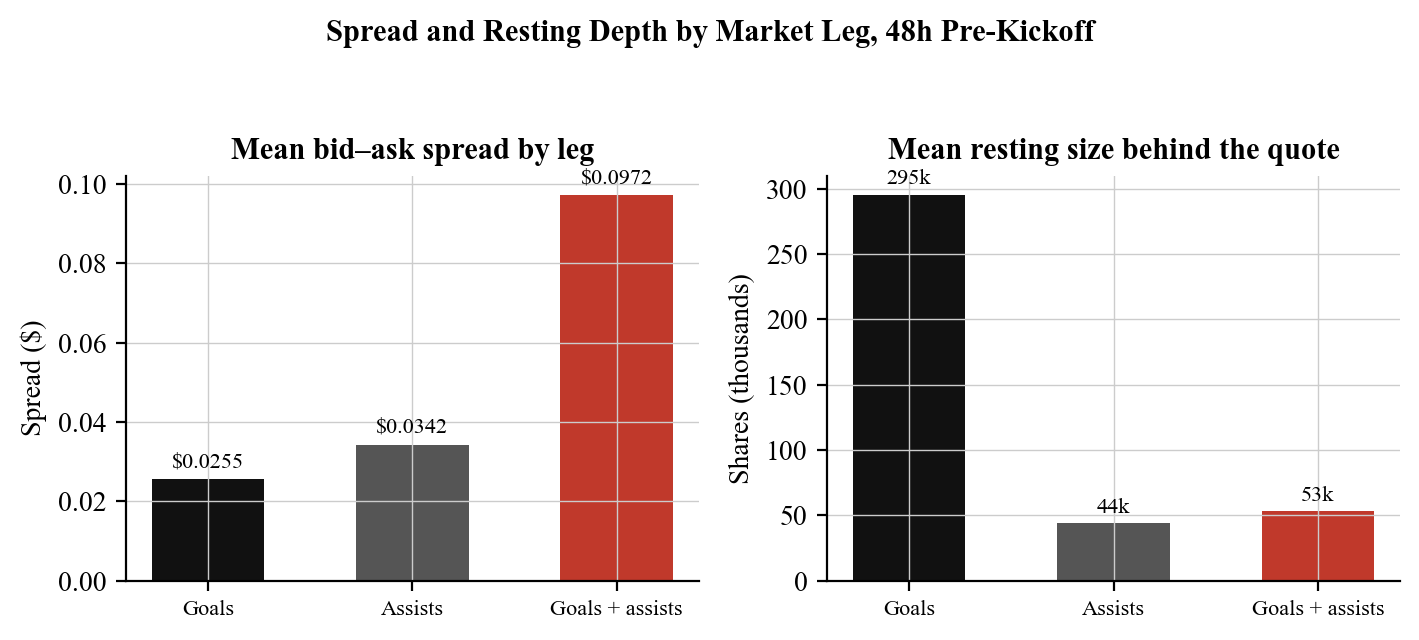
\includegraphics[width=\linewidth]{figures/fig1_spread_depth.png}
\end{center}

The compound contract is the stale one on both measures at once. It carries a
3.81$\times$ wider spread than the goals leg (\$0.0972 against \$0.0255) and
rests 5.6$\times$ less size behind its quotes (52{,}966 against 295{,}156
shares), widening to 7.5$\times$ in the final four hours. The goals leg barely
moves: its spread stays near \$0.019 for the entire two days, and its book grows
from roughly 295{,}000 to 376{,}000 shares as retail money arrives. The compound
market does the opposite. It opens at a \$0.157 spread and compresses to \$0.047
by kickoff, but its resting size never grows. Retail flow goes to the simple
market and largely skips the compound one.

\subsection{Logical-Floor Violation Rate by Time to Kickoff}

The plot below shows the fraction of pre-kickoff observations in which the
compound bid sat below the goals bid, grouped by hours before kickoff.

\begin{center}
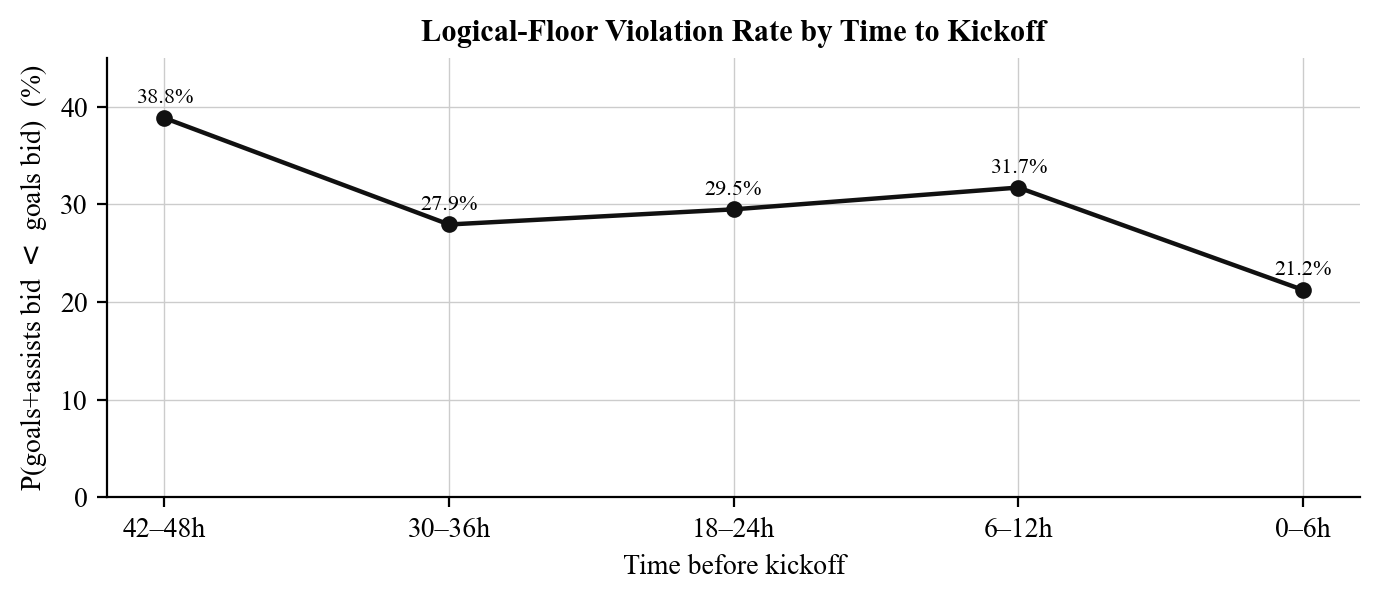
\includegraphics[width=\linewidth]{figures/fig2_violation_decay.png}
\end{center}

The best resting bid on the more likely outcome sat below the best resting bid on
a subset of it in 28.81\% of pre-kickoff observations (35{,}894 of 124{,}571), by
a mean of \$0.088. The violation rate is highest far from kickoff, 38.83\% at
forty-two to forty-eight hours out, and falls to 21.23\% inside the final six
hours, which is what a de-staling process predicts. It also runs opposite to
fame. Messi's compound book violated the identity six times in 7{,}287
observations. Players one tier below the household names, well known enough to
draw flow but not so well known that the compound leg drew the same attention as
the simple one, carried violation rates above 20\%.

\subsection{Mean Absolute Cross-Market Gap by Time to Kickoff}

The plot below tracks the mean absolute difference between the compound price and
its formula fair value, by time bucket, from more than a day before kickoff
through live play.

\begin{center}
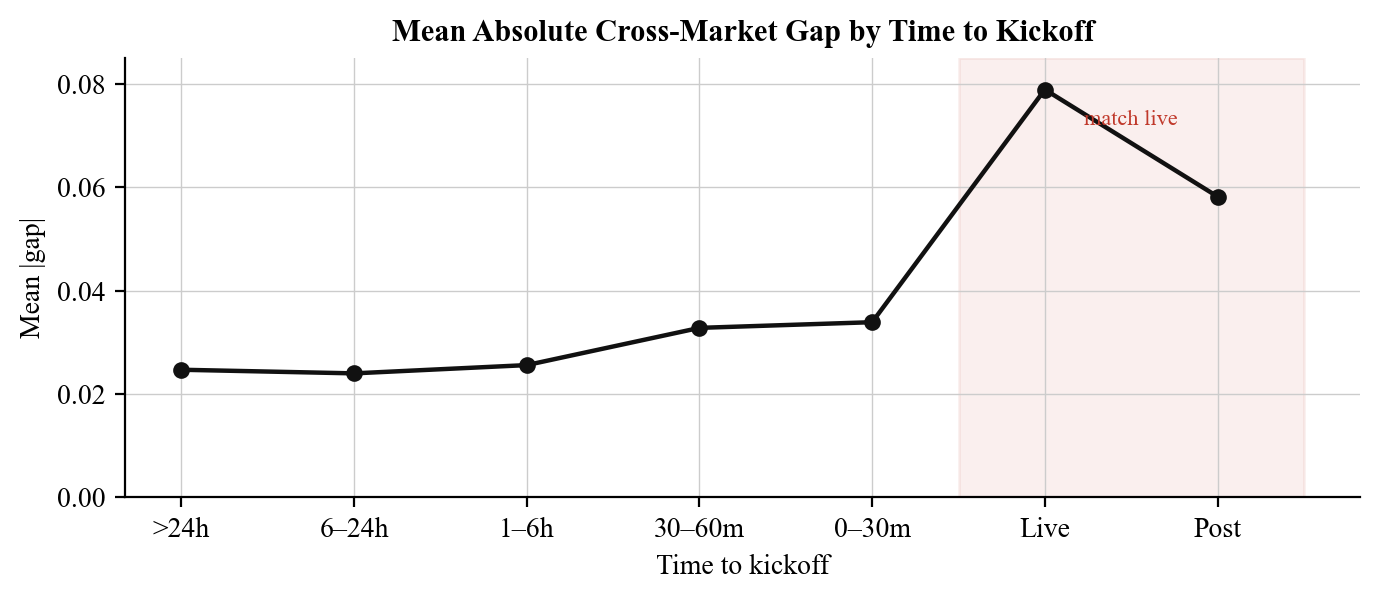
\includegraphics[width=\linewidth]{figures/fig3_gap_by_time.png}
\end{center}

The gap is roughly flat near 0.025 for the entire pre-kickoff window and then
more than triples, to 0.079, once the match goes live. Scoring events reach the
three legs at different speeds, and that lag is what the second strategy trades.

\subsection{Gap Narrowing: Observed vs. Monte Carlo Benchmark}

To check whether the pre-kickoff mispricing reverts rather than just drifts,
per-step increments of \gap\ were computed from 182{,}760 consecutive
same-player, same-game observations (median step about sixty-six seconds), giving
a mean of approximately zero and a standard deviation of $\sigma = 0.0227$ per
step. For each of the twenty-seven cleanly pre-kickoff-exited positions with a
resolvable gap reading at both entry and exit, 5{,}000 random-walk paths were
simulated, each starting at that position's actual entry gap and taking its
actual number of observed steps, and the fraction of paths ending with a smaller
absolute gap than they started with was recorded.

\begin{center}
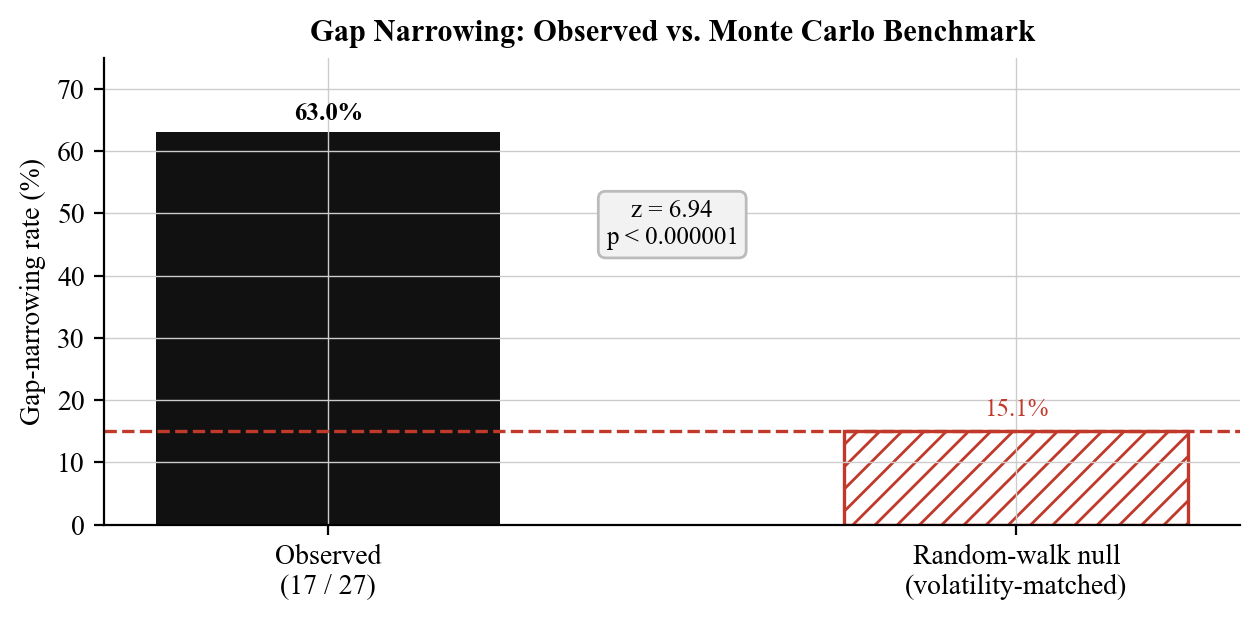
\includegraphics[width=0.86\linewidth]{figures/fig4_meanrev_vs_mc.png}
\end{center}

The observed data narrows far more often than the volatility-matched benchmark:
63.0\% of the real positions closed toward fair value, against 15.1\% of the
simulated paths. The simulation is calibrated from the real step-by-step
movements and has no drift, so the gap between 63\% and 15\% is not an artifact
of a parameter choice.

\section{Statistical Testing}

Each test below is a one-sample proportion $z$-test. Where the null probability
is an entry price rather than a fixed benchmark, the test asks whether the
strategy's realized results differ from what the market's own pricing implied.
That is the right question for a strategy that might just be fast rather than
better informed.

\subsection{Test 1: Is the gap mean-reversion real?}

The null hypothesis is that the gap signal follows a driftless,
volatility-matched random walk, which narrows 15.1\% of the time.
\begin{align*}
H_0:\; p = 0.151 \qquad H_1:\; p > 0.151 \qquad
n = 27, \quad \hat p = 0.630
\end{align*}
\[
z = \frac{0.630 - 0.151}{\sqrt{\dfrac{0.151\,(1 - 0.151)}{27}}} = 6.94,
\qquad p < 0.000001.
\]
The $p$-value is effectively zero, so we reject the null. One caveat: contract
prices live in $[0,1]$, so \gap\ is bounded and the simulated walk is not, and a
bounded process that starts far from zero has to revert eventually because it has
nowhere else to go. Two things limit how much of the result that can explain.
First, the effect is large: a boundary artifact does not plausibly produce a
63.0\% against 15.1\% margin at these gap sizes. Second, the low simulated rate
comes from the walk having room to drift over a typical holding period, not from
the walk being pushed outward. Re-running the null with reflecting barriers at
the price bounds would raise the simulated rate somewhat but would not close the
gap.

\subsection{Test 2: Is the speed strategy calibrated?}

The speed strategy trades a confirmed public event before the resting book
requotes. Which side it ends up holding depends on the event: a confirmed goal or
assist leaves it long ``Yes,'' a confirmed substitution or full-time whistle
leaves it long ``No.'' Both are the same trade, acting on public news faster than
the book adjusts, applied to opposite events, so they are tested together. The
null hypothesis is that the market was already pricing those contracts
efficiently, so the true win probability equals the average price the account
paid for the side it held.
\begin{align*}
H_0:\; p = 0.917 \qquad H_1:\; p \neq 0.917 \qquad
n = 164, \quad \hat p = 0.878
\end{align*}
\[
z = \frac{0.878 - 0.917}{\sqrt{\dfrac{0.917\,(1 - 0.917)}{164}}} = -1.81,
\qquad p = 0.070.
\]

\begin{center}
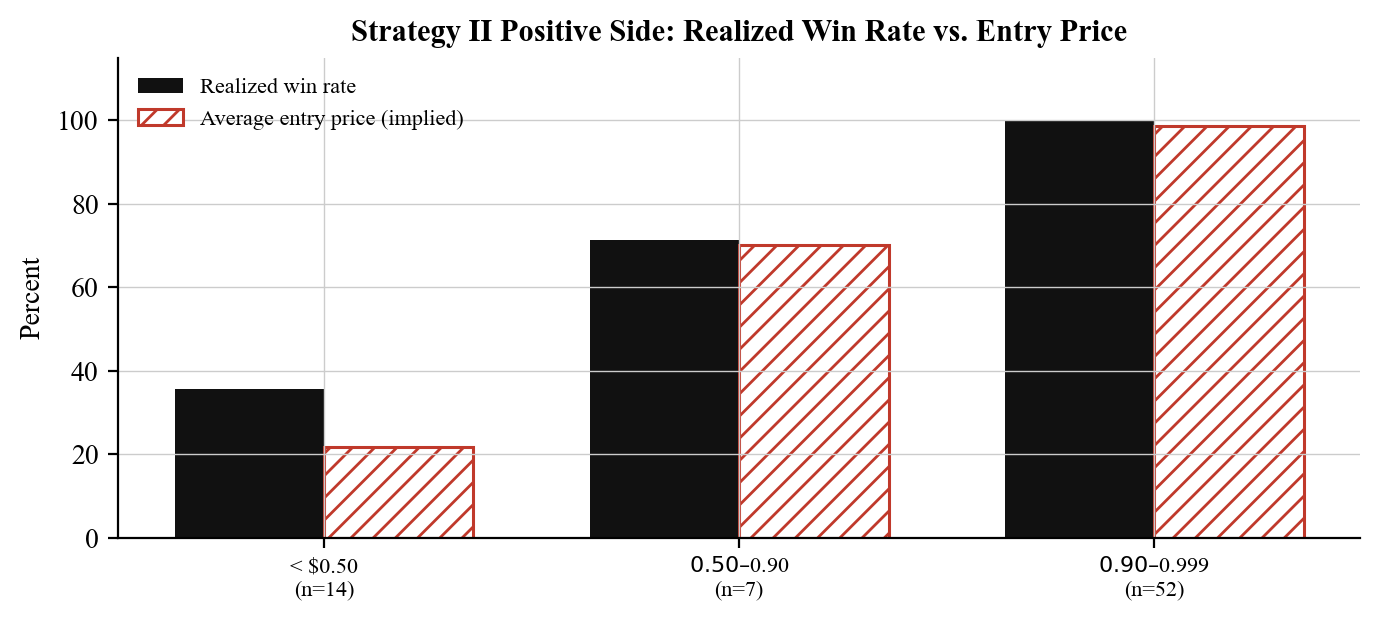
\includegraphics[width=\linewidth]{figures/fig5_calibration.png}
\end{center}

We fail to reject the null, and the shape of the result is more informative than
the failure itself. The 137 positions entered above 90\% implied confidence
resolved the account's way 98.5\% of the time, against a 98.5\% implied rate.
That is calibrated to the decimal, and uninformative for the same reason: buying
a contract the market has priced at 98\% and watching it settle at 98\% is
arithmetic rather than skill. A perfect record in that band carries little
weight; across the 48-position ``Yes'' sub-bucket alone, a flawless outcome has
probability $0.987^{48} \approx 0.53$ under the market's own pricing. The 18
positions entered between 50\% and 90\% implied resolved at 38.9\% against a
74.7\% implied rate. This is a real shortfall, dominated by two positions
(Section 6), with a thin low-confidence tail behind them.

The test is also underpowered against the edge the mechanism actually claims. At
$n = 164$ and a null of 91.7\%, the realized rate would have had to clear roughly
95\% to reject at conventional significance, while Section 7 claims only a
two-to-three-point timing edge. The right reading of $p = 0.070$ is ``no edge
this sample can detect, plus a small miss concentrated in the least-priced
entries,'' not a demonstrated edge in either direction. The speed strategy's
profit is real and mechanically reliable. A win rate just cannot tell whether it
comes from skill or from buying contracts the market had already priced near
certainty.

\subsection{What the win rates do and do not show}

The speed strategy's headline win rate, 87.8\% across its 164 held positions,
invites a reading it cannot support. The strategy buys contracts the market has
already priced between roughly 80\% and 99\% and holds them to settlement, so a
high win rate is what those entry prices predict rather than a result. A
perfectly calibrated market handed the same trades would produce the same number.
The question that separates edge from arithmetic is whether the realized rate
beats the price paid. Test 2 answers it: the realized rate sits just below the
price paid, and the miss is concentrated in a thin band of low-confidence entries
rather than spread across the book. This is not what a strategy that prices
better than the market looks like.

That leaves the speed strategy's profit resting on a timing claim: it buys after
a goal, substitution, or whistle is public but before the resting book requotes.
A win rate cannot establish this, because a stale price and a fair price at 99\%
resolve the same way. The only direct evidence is the reaction-time sample in
Section 2: seven independently timestamped goals, a mean latency near 91 seconds,
every entry landing while the contract still traded below the post-event fact.
Seven observations is a real sample but a thin one, and it is the only evidence
the speed strategy has. Only the patience strategy has an edge that survives a
test against the market's own pricing.

\subsection{Multiple comparisons and in-sample validity}

Bonferroni-correcting the two tests above (threshold $0.05 / 2 = 0.025$)
changes no conclusion: the mean-reversion test clears it by orders of magnitude,
and the speed-strategy calibration test does not reach even the uncorrected
$0.05$. The bigger problem is that the gap signal was designed and evaluated on
the same thirty-five-day dataset, with no out-of-sample holdout. A complete census of every soccer
competition Polymarket US lists finds that none of the other seventy leagues
currently carries the three-parallel-market structure the signal requires, so a
genuine replication needs a second tournament that does not yet exist. The
collector already discovers events across all seventy leagues, so that data
begins accumulating the moment one lists a player goal or assist market again.

\section{Risk}

A key risk to the patience strategy arises when the compound contract's staleness
does not close before kickoff. The exit is a passive resting sell rather than a
market order, so it depends on a counterparty's order arriving. When it does not
fill in time, the position is carried into live play, where match variance sits
on top of an already-late exit. Of 193 round-trip positions, only 56 fully
exited before kickoff as intended; the remaining 137 were carried into the match.
The 56 clean exits won 96.4\% of the time; the 137 delayed positions won only
80.3\%, with lower average returns. That is the cost of fill risk. The clean-exit
number is partly a selection artifact: a position moving the wrong way is more
likely to still be open at kickoff than sold at a loss beforehand.

Jeremy Doku's goals-or-assists position ahead of Belgium--Senegal is one example.
It was bought across three pre-kickoff fills at \$0.29 to \$0.31, a blended
\$0.2978, and was not sold before kickoff. Carried into the match, it filled
across six tranches at \$0.38 to \$0.41, realizing $+\$25.18$ (+27.6\%) and
$+\$23.57$ on its two largest tranches. The mispricing it was entered on was
real. It closed late, and a first move the other way would have produced the
opposite result on the same delay.

The speed strategy carries a different risk on its ``No'' positions: a confirmed
substitution or full-time whistle caps a player's remaining probability, but two
positions were entered well short of certainty and resolved against the call.
Charles De Ketelaere (goals-or-assists, Spain--Belgium, 07-10), entered at an
average ``No'' price near 79\%, lost \$73.47, the largest single-position loss in
the strategy data. Jovo Luki\'c (goals, Bosnia and Herzegovina--Qatar, 06-24),
entered near 88\%, lost \$46.38. Both are signal misses rather than execution
artifacts. They are the two largest dollar losses in the strategy and account for
most of the 50 to 90\% bucket's calibration gap in Test 2. Above 90\% implied,
which is 137 of the strategy's 164 held positions, realized and implied rates
match to within a point.

To keep the latency measurement honest, event timestamps are taken only from
neutral match reports, never from Polymarket's price data, and second-half goals
are excluded rather than approximated. Converting a second-half minute to a
wall-clock time requires the real halftime-break length, and assuming a standard
fifteen minutes can swing a computed latency by 300 seconds, more than the
quantity being measured.

\section{Execution Model}

\subsection{Pre-Trade Identification and Filtering}
\begin{itemize}
\item \textbf{Clean three-leg observation.} A candidate surfaces only when all
three legs quote from the same pre-kickoff market state and the gap exceeds a
threshold; $|\gap| > 0.05$ held on 31 of 208 clean samples.
\item \textbf{Star-player universe.} Positions concentrate on high-coverage names
(Messi, Mbapp\'e, Haaland, Kane and similar), whose compound markets de-stale
reliably enough to exit into before kickoff. An obscure player can carry the same
gap on paper, with far less confidence it closes and far less volume to exit
into.
\end{itemize}

\subsection{Entry Logic}
\begin{itemize}
\item \textbf{The fair-value ceiling.} Rather than crossing the spread, the
patience strategy repeatedly improves its own resting bid in small increments,
capped strictly below the formula-implied fair value, so the position buys at or
below its own fair-value estimate even in the best case for a counterparty. On
the fills, 96.2\% of pre-kickoff compound buys were priced below the formula
value computed from the concurrent leg asks.
\item \textbf{Passive only.} Section 4 shows the inefficiency sat almost entirely
on the bid side. A crossable, locked arbitrage, buying the compound at its ask
and selling the goals leg at its bid, existed in only 0.05\% of observations. An
aggressive strategy would have found nothing to take.
\item \textbf{The confirmed-event trigger.} The speed strategy triggers on
events, not price levels. On a confirmed goal, assist, substitution, or final
whistle for a tracked player, the near-certain side is bought at whatever price
is showing and held to \$1.00 settlement.
\end{itemize}

\subsection{Risk and Position Management}
\begin{itemize}
\item \textbf{Fixed-dollar sizing.} Positions are sized as a fixed fraction of
available capital rather than a share count, for consistency across contract
prices.
\item \textbf{Hard cap.} Total portfolio risk is capped at 5\% of capital,
checked at kickoff; a position built past that fraction across multiple fills is
cut back with a below-market sell.
\item \textbf{Breadth over size.} The speed strategy spreads capital across every
still-unresolved candidate at the moment of the trigger rather than concentrating
on one, since the confirming event makes each outcome close to certain rather
than just likely.
\end{itemize}

\subsection{Exit Strategy}
\begin{itemize}
\item \textbf{Staged sell-off.} Inside the final five minutes before kickoff, the
patience strategy sells roughly a quarter of whatever remains once per minute,
crossing the spread each round to guarantee that tranche fills.
\item \textbf{Unconditional backstop.} A final sweep at kickoff closes anything
the schedule leaves behind, so the position is meant to be flat by kickoff, a
property the trade record found missing in 137 of 193 cases.
\item \textbf{Hold to settlement.} Once a speed-strategy entry lands near \$0.98
to \$0.99, the remaining margin is too thin, net of the trading fee, to be worth
an active sell. Zero of 193 patience-strategy round-trips were ever sold at a
price at or above \$0.90; every position that reached that band was held to
settlement.
\end{itemize}

The live order-placement layer for the patience strategy was developed jointly
with a collaborator on a separate account and is described here as reconstructed
from that logic and cross-checked against the surviving trade ledger; every
figure in this paper derives from the author's own account and its own records.

\section{Final Weights}

Two execution schedules follow from the model above. The pre-kickoff exit, which
exists to close the fill-risk gap in Section 6, sells a fixed fraction of the
remaining position each minute inside the final five, with an unconditional
backstop at kickoff:

\begin{center}
\begin{tabular}{@{}c l c c@{}}
\toprule
Minutes to kickoff & Action & Fraction of remainder & Cumulative \% closed \\
\midrule
5 & Staged sell        & 25\%  & 25.0\% \\
4 & Staged sell        & 25\%  & 43.8\% \\
3 & Staged sell        & 25\%  & 57.8\% \\
2 & Staged sell        & 25\%  & 68.4\% \\
1 & Staged sell        & 25\%  & 76.3\% \\
0 & Unconditional sweep & 100\% & 100\%  \\
\bottomrule
\end{tabular}
\end{center}

Entries are not scheduled the same way. They are placed as the signal appears,
across the full pre-kickoff window. Of 86 pre-kickoff compound buys, the median
fill landed 8.7 hours before kickoff (mean 14.6 hours), and the fills cluster in
two human-scale windows rather than spreading evenly:

\begin{center}
\begin{tabular}{@{}l c@{}}
\toprule
Window before kickoff & Share of pre-kickoff compound buys \\
\midrule
18--24 hours & 20\% \\
6--18 hours  & 37\% \\
Final 6 hours & 43\% \\
\bottomrule
\end{tabular}
\end{center}

\section{Results}

The strategies were run against Polymarket US's World Cup player-prop markets over
a thirty-five-day window, 2026-06-15 to 2026-07-19. Net capital contributed was
\$1{,}200 across four completed deposits; the account carries zero open positions
at close, so every figure reported is fully realized. Total realized profit over
the window was \$671.99, and it has two parts.

The two strategies this paper analyzes account for \$655.27: \$304.64 from the
patience strategy (compound positions actively sold, 193 closes) and \$350.63
from the speed strategy (confirmed-event trades held to settlement, \$319.71 on
the 164 positions carried to the final whistle, plus \$30.92 on 16 closed by an
active buy-to-cover beforehand). The other \$16.72 is the net result of
discretionary trades the account placed in seven bet types outside either
strategy: match futures, advancement, match-winner, spreads, exact score, player
shots, and shots on target, 26 markets across 89 fills, none of them player
goal-or-assist props. These were not produced by either strategy's entry logic,
are not analyzed further, and are excluded from every test and figure below.

Against SPY over the same calendar window (real closes \$754.83 on 2026-06-15,
\$743.29 on the last trading day before the window ended), the two analyzed
strategies returned $+54.6\%$ on contributed capital (\$655.27 on \$1{,}200),
against SPY's $-1.5\%$. The comparison establishes only that the return is not an
artifact of a broad-market tailwind.

\begin{center}
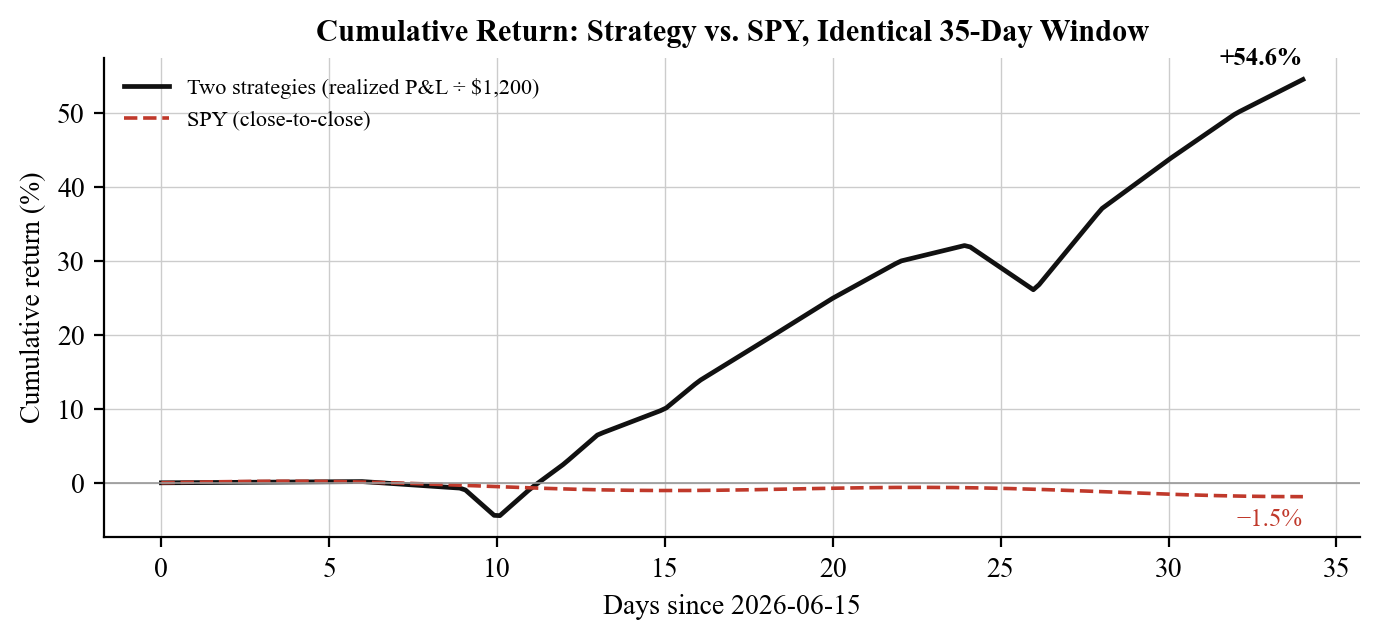
\includegraphics[width=\linewidth]{figures/fig6_cumret.png}
\end{center}

The two strategies behave differently, and only one carries a statistically
validated edge:

\begin{center}
\begin{tabular}{@{}l c c@{}}
\toprule
& Patience (sold) & Speed strategy (held) \\
\midrule
Positions        & 193        & 164 \\
Win rate         & 85.0\%     & 87.8\% \\
Net P\&L         & $+\$304.64$ & $+\$319.71$ \\
Validated edge?  & Yes ($p<0.000001$) & No ($p=0.070$) \\
\bottomrule
\end{tabular}
\end{center}

The speed row covers the 164 positions held to settlement, on which the
calibration test is run; the strategy realized a further \$30.92 on 16 positions
closed by buy-to-cover beforehand, for a total of \$350.63 as broken out above.
The win-rate row is there for completeness but tells you almost nothing about the
speed strategy: it bought contracts the market had already priced between 80\%
and 99\%, so a high win rate is what those entry prices predict rather than a
result (Section 5). The ``validated edge'' row is the one that separates the
two, and only the patience strategy clears it.

Within the patience strategy, the fill-risk split is the more informative
comparison: the 56 positions that exited before kickoff won 96.4\% of the time,
and the 137 carried into live play won 80.3\%.

\begin{center}
\begin{tabular}{@{}l c c@{}}
\toprule
Metric & Strategy & Benchmark (SPY) \\
\midrule
Cumulative return, 35 days   & $+54.6\%$ & $-1.5\%$ \\
Sharpe ratio, daily ($n=31$) & 0.42      & n/a \\
Maximum drawdown             & \$73.94 (11.9\% of peak) & n/a \\
\bottomrule
\end{tabular}
\end{center}

The annualized Sharpe is deliberately not reported. Thirty-one daily observations
from a single bounded event put a wide confidence interval on the daily estimate,
and scaling that interval by $\sqrt{365}$ produces a range wide enough to be
uninformative while still looking precise. Restricting the calculation to the
period after all \$1{,}200 was deposited gives a daily Sharpe of 0.57 on $n=23$,
higher rather than lower once the low-capital ramp-up is removed.

\subsection{Capacity}

The clearest fact in the data about whether this generalizes is that capital grew
as opportunity shrank.

\begin{center}
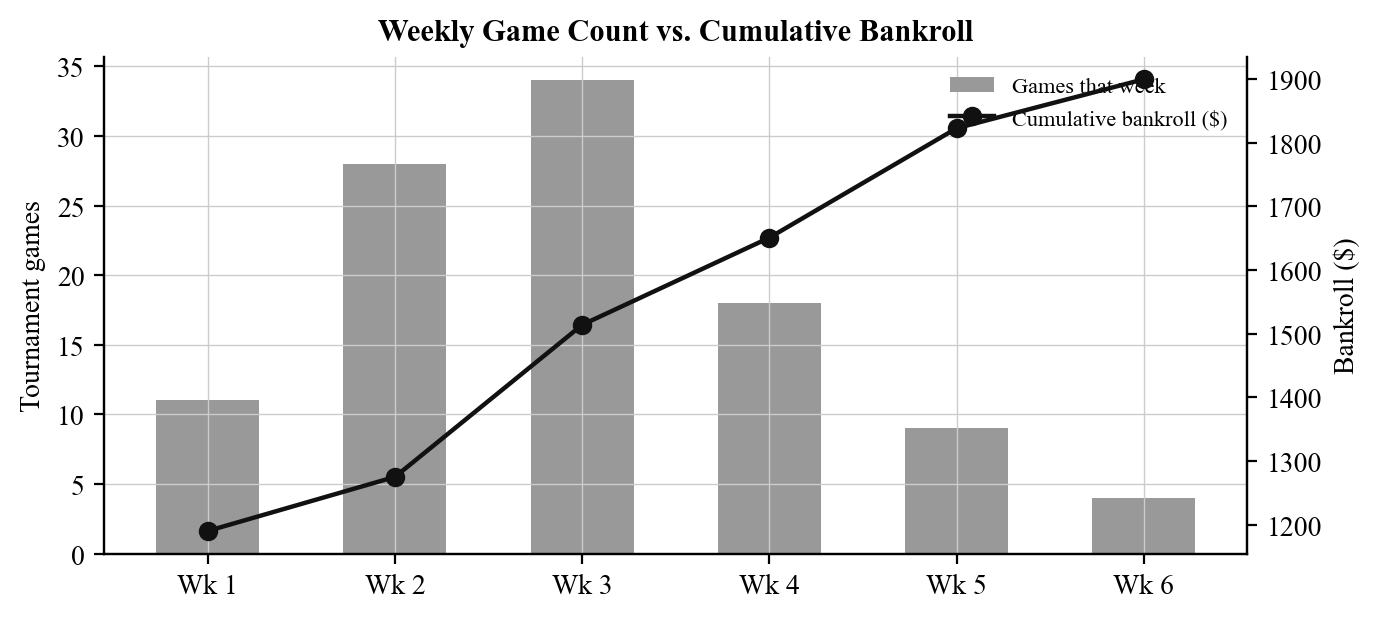
\includegraphics[width=\linewidth]{figures/fig7_capacity.png}
\end{center}

Weekly tournament game count ran 11, 28, 34, 18, 9, 4 as the bracket narrowed,
while the account's bankroll rose steadily from roughly \$1{,}190 to \$1{,}823
across those same weeks. The account held the least capital when opportunity was
greatest and the most when it was smallest. With top-of-book depth of 1{,}406 to
9{,}762 shares against an average position size of \$17.98, and a median
thirty-eight-minute lag between a game-ending event and the settlement that frees
the capital, the strategy is capacity-bound by construction.

\section{Conclusion}

A thinly quoted compound prediction-market contract, priced against the more
active single-stat contracts that decompose it, carries a mechanical pricing
inefficiency. Its bid falls below the logical floor
$P(\text{goal} \cup \text{assist}) \geq P(\text{goal})$ in 28.81\% of 124{,}571
pre-kickoff observations, and that staleness reverts toward fair value far more
often than a volatility-matched random walk predicts: 63.0\% against 15.1\%,
$p < 0.000001$. This is the only edge in the paper that survives a test against
the market's own pricing. A second strategy trades confirmed public events
directly. It is profitable, but the results are not evidence of skill: it buys
contracts already priced at 80\% to 99\% and holds them, so a high win rate is
what those prices predict. A calibration test cannot separate it from its own
entry pricing (87.8\% realized against 91.7\% implied, $p = 0.070$), and the
small miss it does show sits in a thin tail of low-confidence entries. Its profit
rests on a timing claim the win rate cannot test, supported by only seven
directly measured event latencies. The account turned \$1{,}200 into \$671.99 of
fully realized profit over thirty-five days: \$655.27 from the two strategies
analyzed here and \$16.72 from discretionary trades outside them. On the strategy
figure that is $+54.6\%$ against SPY's $-1.5\%$ over the same window.

The inefficiency is real, but it is capacity-bound by construction. The account
held the least capital when tournament opportunity was greatest and the most when
it was smallest, and measured book depth against realized position size leaves no
room to scale without redesigning the execution layer. The overall picture is a
retail-heavy prediction market that prices its simple contracts efficiently and
its compound contracts against itself, an asymmetry a faster, better-modeled
counterparty can capture at small size but not, on this evidence, at
institutional scale.

\end{document}
